\documentclass{beamer}

\usepackage{amssymb,amsmath}
\usepackage{graphicx}
\usepackage{url}
\usepackage{color}
\usepackage{relsize}		% For \smaller
\usepackage{url}			% For \url
\usepackage{epstopdf}	% Included EPS files automatically converted to PDF to include with pdflatex

%For MindMaps
% \usepackage{tikz}%
% \usetikzlibrary{mindmap,trees,arrows}%

%%% Color Definitions %%%%%%%%%%%%%%%%%%%%%%%%%%%%%%%%%%%%%%%%%%%%%%%%%%%%%%%%%
%\definecolor{bordercol}{RGB}{40,40,40}
%\definecolor{headercol1}{RGB}{186,215,230}
%\definecolor{headercol2}{RGB}{80,80,80}
%\definecolor{headerfontcol}{RGB}{0,0,0}
%\definecolor{boxcolor}{RGB}{186,215,230}

%%% Save space in lists. Use this after the opening of the list %%%%%%%%%%%%%%%%
%\newcommand{\compresslist}{
%	\setlength{\itemsep}{1pt}
%	\setlength{\parskip}{0pt}
%	\setlength{\parsep}{0pt}
%}

%\setbeameroption{show notes on top}

% You should run 'pdflatex' TWICE, because of TOC issues.

% Rename this file.  A common temptation for first-time slide makers
% is to name it something like ``my_talk.tex'' or
% ``john_doe_talk.tex'' or even ``discrete_math_seminar_talk.tex''.
% You really won't like any of these titles the second time you give a
% talk.  Try naming your tex file something more descriptive, like
% ``riemann_hypothesis_short_proof_talk.tex''.  Even better (in case
% you recycle 99% of a talk, but still want to change a little, and
% retain copies of each), how about
% ``riemann_hypothesis_short_proof_MIT-Colloquium.2000-01-01.tex''?

\mode<presentation>
{
  % A tip: pick a theme you like first, and THEN modify the color theme, and then add math content.
  % Warsaw is the theme selected by default in Beamer's installation sample files.

  %%%%%%%%%%%%%%%%%%%%%%%%%%%% THEME
  %\usetheme{AnnArbor}
  %\usetheme{Antibes}
  %\usetheme{Bergen}
  %\usetheme{Berkeley}		% bem bacana - menu esquerdo
  %\usetheme{Berlin}
  %\usetheme{Boadilla}
  %\usetheme{boxes}
  %\usetheme{CambridgeUS}		% bem bacana - menu superior
  %\usetheme{Copenhagen}
  %\usetheme{Darmstadt}
  %\usetheme{default}
  %\usetheme{Dresden}
  \usetheme{Frankfurt}
  %\usetheme{Goettingen}
  %\usetheme{Hannover}		% bem bacana - menu esquerdo
  %\usetheme{Ilmenau}
  %\usetheme{JuanLesPins}
  %\usetheme{Luebeck}
  %\usetheme{Madrid}		%bacana
  %\usetheme{Malmoe}
  %\usetheme{Marburg}		% bem bacana - menu direito
  %\usetheme{Montpellier}
  %\usetheme{PaloAlto}		% bem bacana - menu esquerdo
  %\usetheme{Pittsburgh}
  %\usetheme{Rochester}		%bacana
  %\usetheme{Singapore}
  %\usetheme{Szeged}
  %\usetheme{Warsaw}

  %%%%%%%%%%%%%%%%%%%%%%%%%%%% COLOR THEME
  %\usecolortheme{albatross}		% azul escuro, massa
  %\usecolortheme{beetle}		% cinza, menu azul
  %\usecolortheme{crane}		% branco e amarelo, massa
  \usecolortheme{default}		% branco, azul clarinho
  %\usecolortheme{dolphin}		% azul e branco, legal
  %\usecolortheme{dove}			% cinza e branco, feio
  %\usecolortheme{fly}			% todo cinza, horrível
  %\usecolortheme{lily}			% parece o default
  %\usecolortheme{orchid}		% azul e branco, ok
  %\usecolortheme{rose}			% branco e violeta-claro, bonito
  %\usecolortheme{seagull}		% cinza, feio
  %\usecolortheme{seahorse}		% nhé, meio feio
  %\usecolortheme{sidebartab}		% Azul, branco, destaque na tab, interessante
  %\usecolortheme{structure}		% bichado
  %\usecolortheme{whale}		% Azul e branco, bem bonito

  %%%%%%%%%%%%%%%%%%%%%%%%%%%% OUTER THEME
  \useoutertheme{default}
  %\useoutertheme{infolines}
  %\useoutertheme{miniframes}
  %\useoutertheme{shadow}
  %\useoutertheme{sidebar}
  %\useoutertheme{smoothbars}
  %\useoutertheme{smoothtree}
  %\useoutertheme{split}
  %\useoutertheme{tree}

  %%%%%%%%%%%%%%%%%%%%%%%%%%%% INNER THEME
  \useinnertheme{circles}
  %\useinnertheme{default}
  %\useinnertheme{inmargin}
  %\useinnertheme{rectangles}
  %\useinnertheme{rounded}

  %%%%%%%%%%%%%%%%%%%%%%%%%%%%%%%%%%%

  \setbeamercovered{invisible} % or whatever (possibly just delete it)
  % To change behavior of \uncover from graying out to totally
  % invisible, can change \setbeamercovered to invisible instead of
  % transparent. apparently there are also 'dynamic' modes that make
  % the amount of graying depend on how long it'll take until the
  % thing is uncovered.

}


% Get rid of nav bar
\beamertemplatenavigationsymbolsempty

% Use short top
%\usepackage[headheight=12pt,footheight=12pt]{beamerthemeboxes}
%\addheadboxtemplate{\color{black}}{
%\hskip0.5cm
%\color{white}
%\insertshortauthor \ \ \ \ 
%\insertframenumber \ \ \ \ \ \ \ 
%\insertsection \ \ \ \ \ \ \ \ \ \ \ \ \ \ \ \ \  \insertsubsection
%\hskip0.5cm}
%\addheadboxtemplate{\color{black}}{
%\color{white}
%\ \ \ \ 
%\insertsection
%}
%\addheadboxtemplate{\color{black}}{
%\color{white}
%\ \ \ \ 
%\insertsubsection
%}

% Insert frame number at bottom of the page.
% \usefoottemplate{\hfil\tiny{\color{black!90}\insertframenumber}} 

\usepackage[english]{babel}
\usepackage[latin1]{inputenc}
\usepackage{subfigure}

\usepackage{times}
\usepackage[T1]{fontenc}

\usepackage{tikz}
\usetikzlibrary{arrows,shapes}
\tikzstyle{vertex}=[circle,fill=black!25,minimum size=10pt,inner sep=0pt]
\tikzstyle{blue vertex}=[circle,fill=blue!100,minimum size=10pt,inner sep=0pt]
\tikzstyle{red vertex}=[circle,fill=red!100,minimum size=10pt,inner sep=0pt]
\tikzstyle{edge} = [draw,thick,-]
\tikzstyle{red edge} = [draw, line width=5pt,-,red!50]
\tikzstyle{black edge} = [draw, line width=5pt,-,black!20]
\tikzstyle{weight} = [font=\smaller]

\title[GB21802]{GB21802 - Programming Challenges}
\subtitle[]{Week 8 - Computational Geometry}
\author[Claus Aranha]{Claus Aranha\\{\footnotesize caranha@cs.tsukuba.ac.jp}}
\institute{College of Information Science}
\date{2019-06-14,17\\{\tiny Last updated \today}}


\begin{document}

\section{Introduction}
\subsection{Title}
\begin{frame}
\maketitle
\end{frame}

% \subsection{Last Class}
%
% \begin{frame}
  \frametitle{Results for the Previous Week}

  \begin{center}
    Here are the results for last week:

    \bigskip
    
    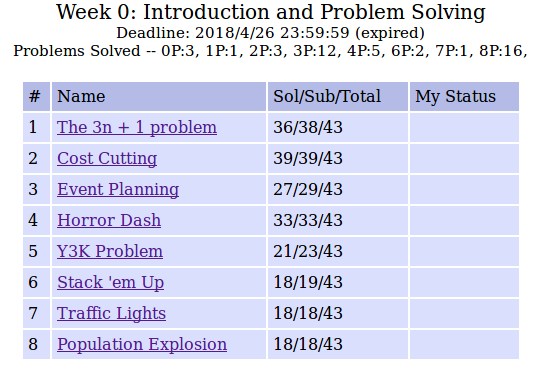
\includegraphics[width=0.8\textwidth]{img/resultW0}
    
    \bigskip

    Hope you enjoyed the warm up!
  \end{center}

\end{frame}

\begin{frame}[fragile]
  \frametitle{Comments from e-mails and questions -- 1}

  \begin{block}{Submission with Java}
    Two students had \structure{``runtime error''} with Java last week
    -- don't forget that your start class MUST be called {\bf Main}.
  \end{block}

  \vfill

\begin{verbatim}
class Main {
  public static void main(String[] args) {

    // do something...

  }
}
\end{verbatim}
\end{frame}

\begin{frame}
  \frametitle{Comments from e-mails and questions -- 2}
  \begin{block}{Input/Output}
    Two other students had problems because their program printed ``Please enter a number''.

    \bigskip

    You are very kind, but please {\bf follow the specifications} strictly!
  \end{block}
  
  \vfill

  \begin{block}{Format for MANABA submission}
    One student asked if the code for MANABA had to be the same as the code for UVA.

    \bigskip

    Yes. The code you submit on MANABA must be {\bf exactly the same}
    as the code you submitted for UVA.
  \end{block}
\end{frame}

\begin{frame}
  \frametitle{Short comments about the problems:}
  \begin{itemize}
  \item Cost Cutting, Event Planning, Horror Dash -- Easiest problems (find mean, find min, find min);
    \bigskip

  \item 3n+1 -- Still easy, but a few traps -- example of {\bf Memoization};
    \bigskip

  \item Y3K Problem -- Still easy, but skip year can be a bit troublesome.
    
  \end{itemize}
\end{frame}

%\begin{frame}
%  \frametitle{Comments about the problems}
%\end{frame}


\subsection{Outline}
\begin{frame}
  \frametitle{Computational Geometry}
  \framesubtitle{What is it?}

  {\small

    \structure{Computational Geometry} problems involve answering
    questions about \structure{lines, points and angles}. Some example
    questions:

    \bigskip

    \begin{block}{}
    \only<1>{Given $N$ points $(s_1, s_2, s_3, \ldots, s_N)$, what is
      the area of the poligon that covers all the points?}

    \only<2>{Given $N$ rectangles, $x_1,y_1,w_1,h_1; \ldots; x_N, y_N,
      w_N, h_N$, what is the length of lines needed to connect them?}

    \only<3>{Given a polygon, and $N$ points, what is the line
      that divides the polygon in equal areas, so that the same
      number of points are in each area?}
    \end{block}

    \begin{center}
      \includegraphics<1>[width=0.8\textwidth]{img/sampleproblem_1.png}
      \includegraphics<2>[width=0.6\textwidth]{img/sampleproblem_2.png}
      \includegraphics<3>[width=0.4\textwidth]{img/sampleproblem_3.png}
    \end{center}

  }
\end{frame}

\begin{frame}
  \frametitle{Computational Geometry}
  \framesubtitle{The good and the bad}

  \begin{itemize}
  \item \structure{Good}: Geometry problems are fun
  \item \structure{Good}: You have to draw pretty pictures
  \item \structure{Good}: Mostly algorithms from high school
  \item \structure{Good}: Code is highly re-usable

    \bigskip

  \item \alert{Bad}: You have to write a lot of code (in the beginning!)
  \item \alert{Bad}: Very easy to get WE...
  \end{itemize}
\end{frame}


\begin{frame}
  \frametitle{Easy Mistakes in Geometry Problems}

  {\small
    \begin{block}{Problem 1 -- Special Cases}
      \begin{itemize}
      \item Multiple points in the same place;
      \item Collinear points;
      \item Vertical lines;
      \item Parallel Lines;
      \item Intersection at end of segment;
      \item etc;
      \end{itemize}
    \end{block}

    \begin{block}{Problem 2 -- Precision Errors}
      \begin{itemize}
      \item Functions require many multiplications and divisions;
      \item Easy to propagate floating point errors;
      \end{itemize}
    \end{block}
  }
\end{frame}


\begin{frame}[fragile]
  \frametitle{Easy Mistakes in Geometry Problems}

  {\smaller

    \begin{block}{Dealing Special Cases}
      \begin{itemize}
      \item Make sure to add special cases to your
        library functions;
      \end{itemize}
    \end{block}

    \begin{block}{Solving Precision Errors}
      \begin{itemize}
      \item If possible, convert all values to integers
      \item Use an EPSILON constant for comparisons:

\begin{verbatim}
if (float.1 == float.2) then            // NO
if (fabs(float.1 - float.2) < EPS) then // YES!
\end{verbatim}

      \end{itemize}
    \end{block}
  }
\end{frame}

\begin{frame}
  \frametitle{Class Outline}
  \begin{itemize}
  \item Example Problems;
  \item Basic Geometric Functions;
  \item Circles;
  \item Triangles;
  \item Polygons;
  \end{itemize}
\end{frame}



\section{Basic Functions}

\subsection{Problem Example -- 1}
\begin{frame}
  \frametitle{Problem Example: UVA 191 -- Intersection}

  {\small
    \begin{block}{Summary}
      \begin{itemize}
      \item {\bf Input}\\
        A rectangle and a line:\\
        xstart ystart xend yend xleft ytop xright ybottom

      \item {\bf Output}\\
        T - if the line intersects the rectangle\\
        F - if the line does not intersect the rectangle\\
      \end{itemize}
    \end{block}

    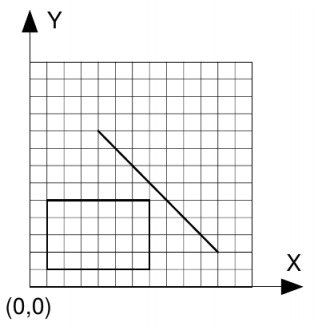
\includegraphics[width=0.35\textwidth]{img/intersection_uva}
    }
\end{frame}

\begin{frame}
  \frametitle{Problem Example: UVA 191 -- Intersection}

  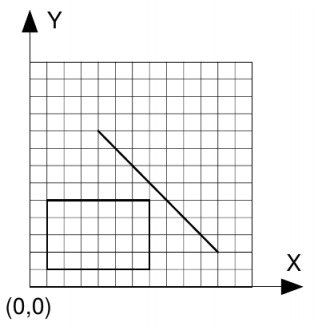
\includegraphics[width=0.45\textwidth]{img/intersection_uva}

  \bigskip
    % TODO: Add code side by side with image
  Steps to calculate the solution:


  \begin{itemize}
  \item Test if $p_1$ or $p_2$ are inside the rectangle;
  \item Test if the segment intersects a side of the rectangle;
  \item (optional) make a bullet hell game;
  \end{itemize}

\end{frame}

\subsection{Problem Example -- 2}

\begin{frame}
  \frametitle{Problem Example: UVA -- Waterfalls}
  {\small
    \begin{block}{Summary}
      \begin{itemize}
      \item {\bf Input}\\
        List of line segments in the waterfall\\
        List of water sources
      \item {\bf Output}\\
        X position where each water source falls\\
      \end{itemize}
    \end{block}

    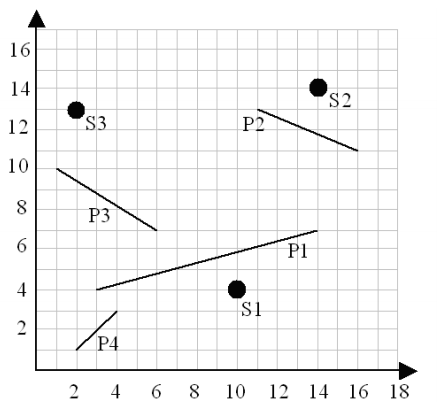
\includegraphics[width=0.4\textwidth]{img/waterfall}
  }
\end{frame}
\begin{frame}
  \frametitle{Problem Example: UVA 833 -- Waterfalls}

  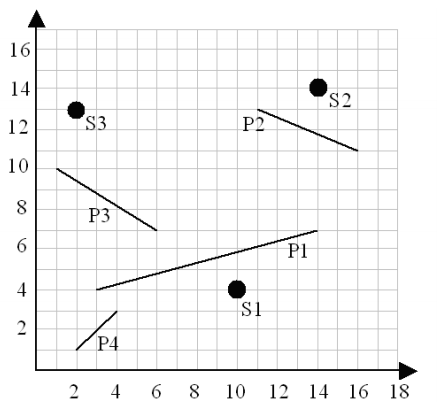
\includegraphics[width=0.4\textwidth]{img/waterfall}

  {\smaller
  For each water source:
  \begin{itemize}
  \item Identify all segments that it intersects with;
  \item Select the highest segment;
  \item Move the source to the bottom of the segment;
  \item Repeat;
  \end{itemize}

  \begin{block}{}
    Many opportunities for pruning and pre-computing! (if necessary)
  \end{block}
  }
\end{frame}

\subsection{Points}
\begin{frame}[fragile]
  \frametitle{Implementing Graphical Problems}
  \framesubtitle{Point Representation}

  {\smaller
    \begin{columns}
      \column{0.6\textwidth}
      \column{0.4\textwidth}
      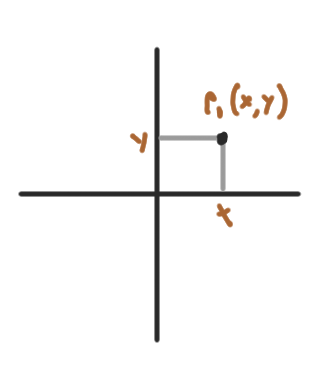
\includegraphics[width=.65\textwidth]{../img/geom2}
    \end{columns}

    \begin{exampleblock}{Point Representation}
\begin{verbatim}
struct point_i { int x, y;  // Using int coordinates.
  point_i() { x = y = 0; }
  point_i(int _x, int _y) : x(_x), y(_y) {}};

struct point { double x, y; // Using floats
  point() { x = y = 0.0;}
  point(double _x, double _y) : x(_x), y(_y) {}};
\end{verbatim}
    \end{exampleblock}
  }
\end{frame}

\begin{frame}[fragile]
  \frametitle{Implementing Graphical Problems}
  \framesubtitle{Comparing and Sorting Points}

  {\smaller

    \begin{exampleblock}{Point Comparison}
\begin{verbatim}
struct point { double x, y;
   point() { x = y = 0.0;
   point(double _x, double _y) : x(_x), y(_y) {}

   // Sorting by coordinate
   bool operator < (point other) const {
      if (fabs(x - other.x) > EPS)
         return x < other.x;
      return y < other.y; }

   // Equality testing -- Note the use of EPS
   bool operator == (point other) const {
      return (fabs(x - other.x) < EPS &&
             (fabs(y - other.y) < EPS)); }
   }
\end{verbatim}
    \end{exampleblock}
  }
\end{frame}

\begin{frame}[fragile]
  \frametitle{Basic Library -- Points 3}
  {\smaller

    Most common distance measure: Euclidean distance. Sometimes
    Manhattan distance (Taxicab distance) is also used.

    \begin{exampleblock}{}
\begin{verbatim}
#define hypot(dx,dy) sqrt(dx*dx + dy*dy)

double dist(point p1, point p2) {
  return hypot(p1.x - p2.x, p1.y - p2.y); }

double taxicab(point p1, point p2) {
  return fabs(p1.x - p2.x) + fabs(p1.y - p2.y); }
\end{verbatim}
    \end{exampleblock}

    \begin{center}
      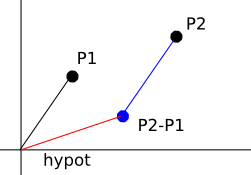
\includegraphics[width=0.5\textwidth]{../img/geom1}
    \end{center}
  }
\end{frame}

\begin{frame}[fragile]
  \frametitle{Basic Library -- Points 4}

  {\smaller

    \begin{exampleblock}{Rotating a point around the origin}
\begin{verbatim}
#define PI           3.14159265358979323846 // Pi const
double PI = 2 * acos(0.0)                   // Better Pi
#define DEG_to_RAD(X) (X*PI)/180.0

// theta is in degrees
point rotate(point p, double theta) {
   double rad = DEG_to_RAD(theta);
   return point(p.x * cos(rad) - p.y * sin(rad),
                p.x * sin(rad) + p.y * cos(rad));}
\end{verbatim}
    \end{exampleblock}
    \begin{center}
      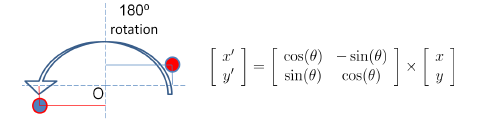
\includegraphics[width=0.8\textwidth]{../img/rotation_halim}
    \end{center}

    {\bf Quiz:} What do you do if you want to rotate a point around $x_0, y_0$?
  }
\end{frame}

\subsection{Lines}

\begin{frame}[fragile]
  \frametitle{Basic Library -- Lines 1}

  {\small
  There are many ways to specify a line:

  \begin{itemize}
  \item \structure{$ax + by + c = 0$} -- useful for most cases.
  \item \structure{$y = mx + c$} -- useful for angle manipulation, but special cases
  \item \structure{$x_0,y_0,x_1,y_1$} -- two points, not very useful for programming.
  \end{itemize}

  \begin{exampleblock}{Point to Line}
\begin{verbatim}
struct line { double a,b,c; };

void pointsToLine(point p1, point p2, line &l) {
   if (fabs(p1.x - p2.x) < EPS {
      l.a = 1.0; l.b = 0.0; l.c = -p1.x; }
   else {
      l.a = -(double) (p1.y - p2.y)/(p1.x - p2.x);
      l.b = 1.0; l.c = -(double) (l.a*p1.x) - p1.y;}
}
\end{verbatim}
  \end{exampleblock}
  }
\end{frame}

\begin{frame}[fragile]
  \frametitle{Basic Library -- Line 2}
  {\smaller

    \begin{columns}
      \column{0.6\textwidth}
      \begin{itemize}
      \item Two lines are parallel if their coefficients $(a, b)$ are the same;
      \item Two lines are identical if all coefficients $(a,b,c)$ are the same;
      \item Remember that we force $b$ to be 0 or 1;
      \end{itemize}
      \column{0.4\textwidth}
      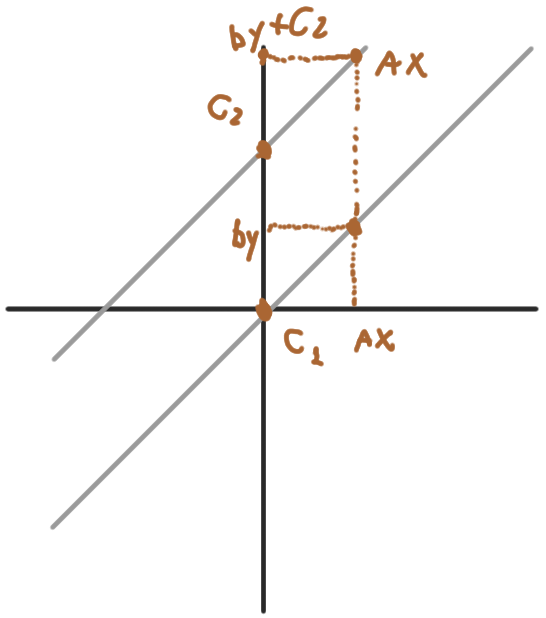
\includegraphics[width=.7\textwidth]{../img/geom3}
    \end{columns}
  \begin{exampleblock}{Parallel and identical lines}
\begin{verbatim}
bool areParallel(line l1, line l2) {
   return (fabs(l1.a-l2.a) < EPS) &&
          (fabs(l1.b-l2.b) < EPS); }

bool areSame(line l1, line l2) {
   return areParallel(l1,l2) &&
          (fabs(l1.c - l2.c) < EPS); }
\end{verbatim}
  \end{exampleblock}
  }
\end{frame}

\begin{frame}[fragile]
  \frametitle{Basic Library -- Line 3}

  {\smaller

    The {\bf intersection} point $x_I, y_I$ is where two lines
    meet. We can find this point by solving the following system of
    linear equations:

    \begin{eqnarray*}
      a_1x+b_1y+c_1 = 0\\a_2x+b_2y+c_2 = 0
    \end{eqnarray*}

    \vfill

    \begin{exampleblock}{Computing the intersection}
\begin{verbatim}
bool areIntersect(line l1, line l2, point &p) {
   if (areParallel(l1,l2)) return False;

   p.x = (l2.b * l1.c - l1.b * l2.c) /
         (l2.a * l1.b - l1.a * l2.b);
   if (fabs(l1.b) > EPS) // Testing for vertical case
      p.y = -(l1.a * p.x + l1.c);
   else
      p.y = -(l2.a * p.x + l2.c);
   return true; }}
\end{verbatim}
    \end{exampleblock}

  }
\end{frame}

\subsection{Segments}
\begin{frame}[fragile]
  \frametitle{Basic Library -- Vectors}
  {\smaller
    \begin{columns}
      \column{0.8\textwidth}
      \begin{itemize}
      \item A \structure{Vector} indicates direction and length;
      \item Represented as a $x,y$ point in relation to the origin;
      \item Operations: Scale, Translation, Addition, Product;
      \end{itemize}
      \column{0.3\textwidth}
      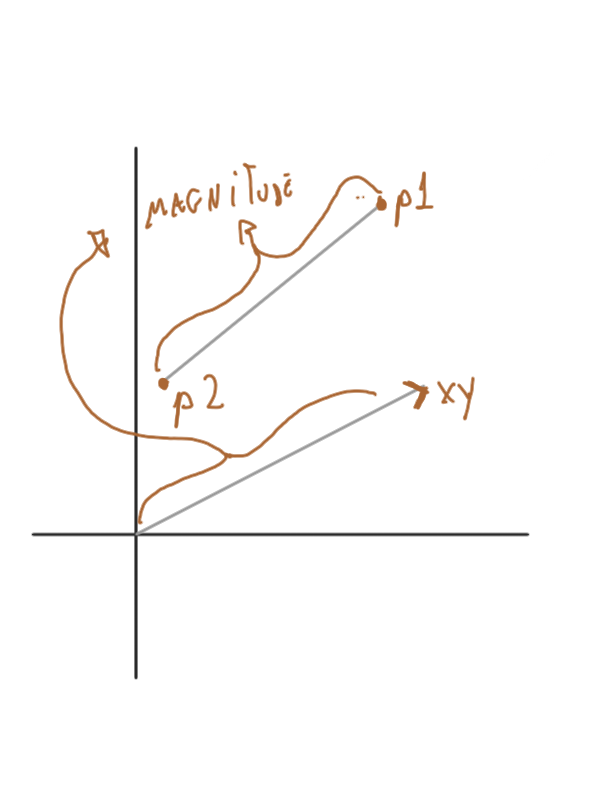
\includegraphics[width=.9\textwidth]{../img/geom4}
    \end{columns}
    \begin{exampleblock}{}
\begin{verbatim}
struct vec { double x, y;
    vec(double _x, double _y) : x(_x), y(_y) {} };

vec toVec(point a, point b) {
    return vec(b.x - a.x, b.y - a.y); }
vec scale(vec v, double s) {
    return vec(v.x * s, v.y * s); }
point translate(point p, vec v) {
    return point(p.x + v.x , p.y + v.y); }
\end{verbatim}
    \end{exampleblock}
  }
\end{frame}

\begin{frame}
  \frametitle{Distance between point and line}
  \begin{block}{}
    Given a point $p$ and a line $l$, the distance between the point
    and the line is the distance between $p$ and the $c$, the closest
    point in $l$ to $p$.

    \bigskip

    We can calculate the position of $c$ by taking the projection of
    $\bar{ac}$ into $l$ ($a,b$ are points in $l$).
  \end{block}

  \begin{center}
    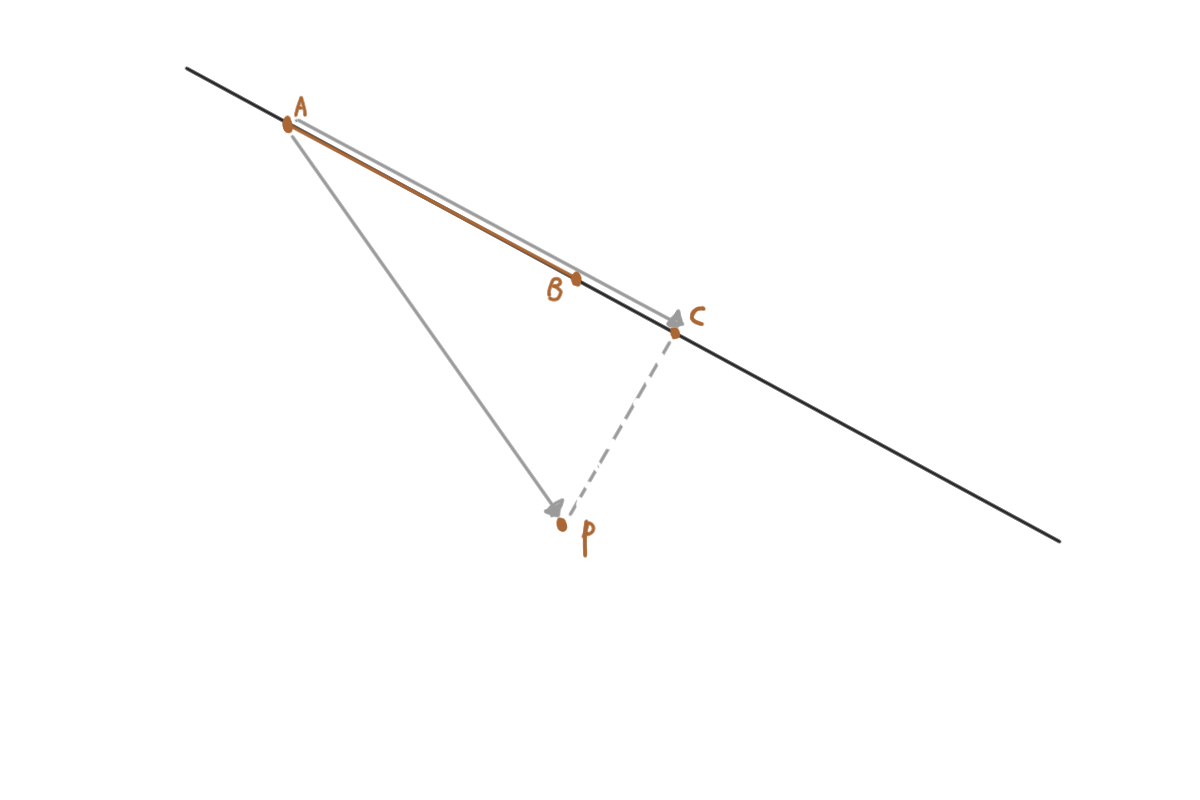
\includegraphics[width=0.8\textwidth]{../img/geom5}
  \end{center}
\end{frame}

\begin{frame}[fragile]
  \frametitle{Distance between point and line}

  {\smaller
  \begin{exampleblock}{}
\begin{verbatim}
double dot(vec a, vec b) {
   return (a.x * b.x + a.y * b.y); }
double norm_sq(vec v) {
   return v.x * v.x + v.y * v.y; }

// Calculates distance of p from line, given
// a,b different points in the line.
double distToLine(point p, point a, point b, point &c) {
  // formula: c = a + u * ab
  vec ap = toVec(a, p), ab = toVec(a, b);
  double u = dot(ap, ab) / norm_sq(ab);
  c = translate(a, scale(ab, u));
  // translate a to c
  return dist(p, c); }
\end{verbatim}
  \end{exampleblock}

}
\end{frame}

\begin{frame}[fragile]
  \frametitle{Distance between point and segment}
  % TODO: Add an image explaining the u conditional
  % TODO: This is actually distance between point and segment. FIX.

  {\smaller
    If we have a \structure{segment} $ab$ instead of a line, the
    procedure to calculate the distance is similar, but we need to
    test if the intersection point falls in the segment.

    \begin{exampleblock}{}
\begin{verbatim}
double distToLineSegment(point p, point a,
                         point b, point &c) {
  vec ap = toVec(a, p), ab = toVec(a, b);
  double u = dot(ap, ab) / norm_sq(ab);

  if (u < 0.0) { c = point(a.x, a.y); // closer to a
                 return dist(p, a); }
  if (u > 1.0) { c = point(b.x, b.y); // closer to b
                 return dist(p, b); }

  return distToLine(p, a, b, c); }
\end{verbatim}
    \end{exampleblock}
  }
\end{frame}

\begin{frame}[fragile]
  % TODO: Explain why angle between segment works
  % TODO: Make appropriate picture to illustrate angle btw segments
  \frametitle{Angles between segments}
  {\smaller

    \begin{exampleblock}{angle between two segments ao and ob}
\begin{verbatim}
#import <cmath>

double angle(point a, point o, point b) { // in radians
vec oa = toVector(o, a), ob = toVector(o, b);
return acos(dot(oa, ob)/sqrt(norm_sq(oa)*norm_sq(ob)));}
\end{verbatim}
    \end{exampleblock}

\structure{Left/Right test}: We can calculate the position of point
$p$ in relation to a line $l$ using the \structure{cross product}.

\smallskip

Take $q,r$ points in $l$. Magnitude of the cross product $pq$ x $pr$
being positive/zero/negative means that $p \rightarrow q \rightarrow
r$ is a left turn/collinear/right turn.

\begin{exampleblock}{}
\begin{verbatim}
double cross(vec a, vec b) {
  return a.x * b.y - a.y * b.x; }
bool ccw(point p, point q, point r) {
  return cross(toVec(p, q), toVec(p, r)) > 0; }
collinear(point p, point q, point r) {
  return fabs(cross(toVec(p, q), toVec(p, r))) < EPS;
\end{verbatim}
\end{exampleblock}
}
\end{frame}


\section{Circles and Triangles}
\subsection{Problem Example}
\begin{frame}
  \frametitle{Problem Example: UVA 10589 Area}

  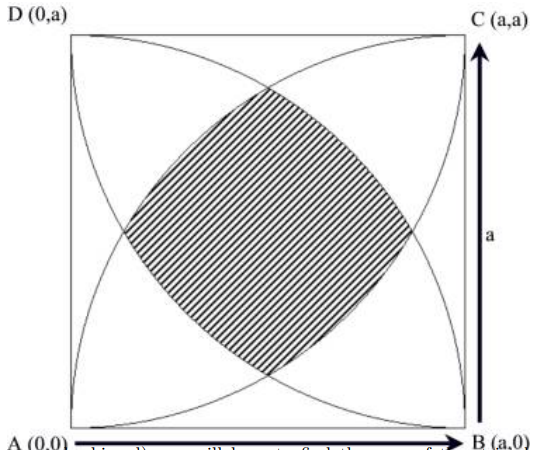
\includegraphics[width=0.4\textwidth]{img/area_uva}

  \begin{block}{}
    \begin{itemize}
    \item What is the area of the shaded part of the rectangle?
    \item You are given the radius of 4 circles, each centered
      in the corners of the rectangle.
    \end{itemize}
  \end{block}

\end{frame}

\subsection{Circles}
\begin{frame}[fragile]
  \frametitle{Circles}
  {\smaller
  \begin{itemize}
  \item A circle is defined by its center $(a,b)$ an its radius $r$
  \item The circle contains all points such $(x,y)$ such as $(x-a)^2+(y-b)^2 \leq r^2$
  \end{itemize}

  \begin{exampleblock}{}
\begin{verbatim}
int insideCircle(point_i p, point_i c, int r) {
   int dx = p.x-c.x, dy = p.y-c.y;
   int Euc = dx*dx + dy*dy, rSq = r*r;
   return Euc < rSq ? 0 : Euc == rSq ? 1 : 2;
   // 0 - inside, 1 - border, 2- outside
}
\end{verbatim}
  \end{exampleblock}
  }
\end{frame}


\begin{frame}
  \frametitle{Circles (2)}
  {\small

    \begin{center}
      % TODO: Make my own image
      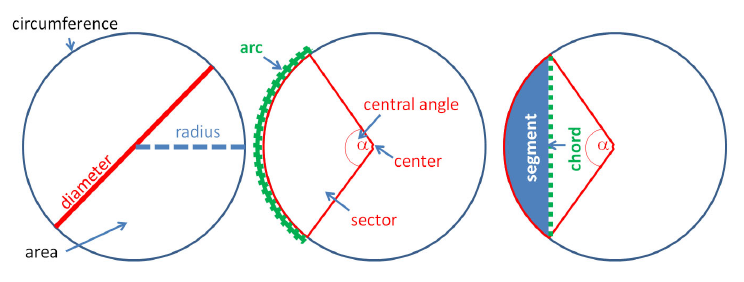
\includegraphics[width=0.85\textwidth]{../img/circle_halim}
    \end{center}

    \begin{itemize}
      \item If you are not given $\pi$, use $pi = 2*$acos$(0.0)$;
      \item Diameter: $D=2r$; Perimeter/Circumference: $C=2\pi r$; Area: $A=\pi r^2$;
      \item To calculat the \structure{Arc} of an angle $\alpha$ (in Degrees), $\frac{\alpha}{360}*C$;
    \end{itemize}
  }
\end{frame}

\begin{frame}
  \frametitle{Circles (3)}
  {\smaller
    \begin{center}
      % TODO: Make my own image, explain why these circles work.
      % TODO: If I have 2 points on a circle, how do I calculate the angle between them?
      %
      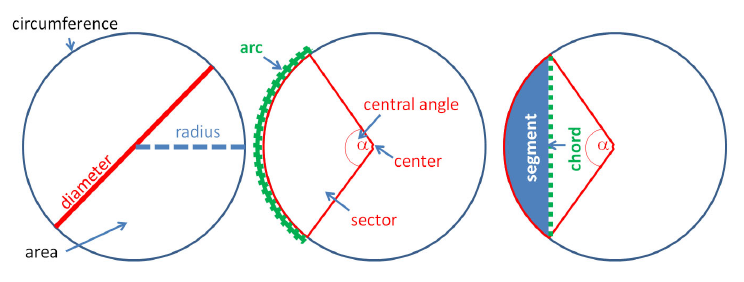
\includegraphics[width=0.75\textwidth]{../img/circle_halim}
    \end{center}

  \begin{itemize}
  \item A \structure{chord} of a circle is a segment composed of two points in the circle's border. A circle with radius $r$ and angle $\alpha$ degrees has a chord of length sqrt$(2r^2(1-\cos{\alpha}))$
  \item A \structure{Sector} is the area of the circle that is enclosed by two radius and and arc between them. Area is: $\frac{\alpha}{360}A$
  \item A \structure{Segment} is the region enclosed by a chord and an arc.

  \end{itemize}
  }
\end{frame}






\subsection{Triangles}

\begin{frame}
  \frametitle{Example: UVA 11909 - Soya milk}
  \begin{block}{}
    \begin{itemize}
    \item {\bf Input}:\\
      The dimensions of a Milk box, and its inclination:\\
      $l, w, h, \theta$
    \item {\bf Output}:\\
      The amount of milk left in the box.
    \end{itemize}
  \end{block}

  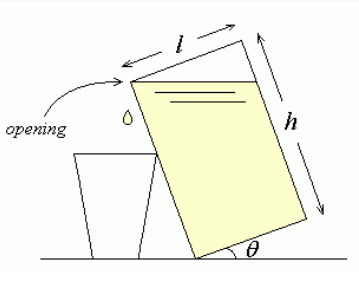
\includegraphics[width=0.4\textwidth]{img/milk_uva}
\end{frame}

\begin{frame}
  \frametitle{Example: UVA 10577 - Bounding Box}
  \begin{block}{}
    Given three vertices of a \structure{regular} polygon,
    calculate the minimal square necessary to cover the polygon.
  \end{block}


  \bigskip

  {\smaller

    \structure{Hint:} You don't actually need to calculate any polygons
  }
\end{frame}

\begin{frame}
  \frametitle{Triangle Basics}
  {\smaller
    Any 2 dimensional polygon can be expressed as a combination of
    triangles. So triangles are important constructs in computational
    geometry.

    \begin{block}{Common Characteristics}
      \begin{itemize}
      \item \structure{Triangle Inequality}: Sides $a,b,c$ obey $a+b > c$
      \item \structure{Triangle Area}: Be $b$ one side of the triangle
        and $h$ its height, $A=0.5bh$
      \item \structure{Perimeter}: $p=a+b+c$
      \item \structure{Semiperimeter}: $s = 0.5p$
      \end{itemize}
    \end{block}

    \begin{block}{Heron's Formula}
      We can calculate the area of a triangle based on its sides:

      \begin{equation*}
        A = \sqrt{s(s-a)(s-b)(s-c)}
      \end{equation*}
    \end{block}


  }
\end{frame}

% TODO: Visual explanation of Heron's formula
\subsection{incircle}
\begin{frame}[fragile]
  \frametitle{Incircle Triangle}
  {\smaller
    % TODO: Add own image of incircle and outcircle triangles
    % TODO: Explain how the calculations for the incircle work
    \begin{columns}
      \column{0.2\textwidth}
      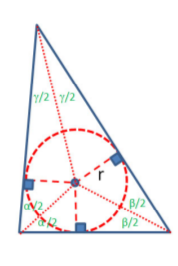
\includegraphics[width=1\textwidth]{../img/incircle_halim}
      \column{0.8\textwidth}

      \begin{exampleblock}{Radius of the Incircle: $r = \text{area}(\Delta)/s$}
\begin{verbatim}
def radiusInCircle(p1,p2,p3):
   ab, bc, cd = dist(p1,p2),dist(p2,p3),
                     dist(p3,p1)
   A = area(ab,bc,ca) % Heron's formula
   P = ab+bc+ca
   return A/(0.5*P)
\end{verbatim}

      \end{exampleblock}
      \end{columns}

    \begin{exampleblock}{Finding the center point of the Incircle}

      \begin{itemize}
      \item Check that the three points are not colinear;
      \item Find the bisection $AP$ of the $AB$-$AC$ angle;
        \begin{itemize}
          {\smaller
          \item Calculate the point $P$ in $BC$ that bisects $A$
          \item The proportion of $BP$ is $(AB/AC)/(1+AB/AC)$
          }
        \end{itemize}
      \item Find the bisection $BP'$ of the $BA$-$BC$ angle;
      \item Fint the intersection of $AP$-$BP'$
      \end{itemize}

    \end{exampleblock}
  }
\end{frame}

\begin{frame}[fragile]
  \frametitle{Incircle Triangle}
  {\smaller
    \begin{exampleblock}{Calculating the Center (Code)}
\begin{verbatim}
int inCircle(point p1, point p2, point p3,
             point &ctr, double &r) {
  r = rInCircle(p1, p2, p3);
  if (fabs(r) < EPS) return 0; // colinear points;
  line l1, l2; // compute these two angle bisectors
  double ratio = dist(p1, p2) / dist(p1, p3);
  point p = translate(p2, scale(toVec(p2, p3),
                      ratio / (1 + ratio)));
  pointsToLine(p1, p, l1);
  ratio = dist(p2, p1) / dist(p2, p3);
  p = translate(p1, scale(toVec(p1, p3),
                ratio / (1 + ratio)));
  pointsToLine(p2, p, l2);
  areIntersect(l1, l2, ctr);
  return 1; }
\end{verbatim}
    \end{exampleblock}
    }
\end{frame}

\subsection{Excircle Triangle}
\begin{frame}
  \frametitle{Excircle Triangle}
  {\smaller
  \begin{columns}
    \column{0.3\textwidth}
    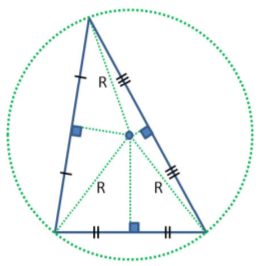
\includegraphics[width=1\textwidth]{../img/circumcircle_halim}
    \column{0.7\textwidth}
    \begin{block}{Radius of the excircle}
      A triangle with sides $a,b,c$ and area $A$ has an excircle with
      radius: $R = abc/4A$.

      \medskip

      The center of the excircle is the intersection of the
      \emph{perpendicular bisectors}.
    \end{block}
    \end{columns}
  \begin{block}{Trigonometry}
    \begin{itemize}
    \item Law of Cosines:\\
      $c^2 = a^2 + b^2 - 2ab\cos{(\gamma)}$\\
      $\gamma = \text{acos}((a^2+b^2-c^2/2ab) $
    \item Law of Sines: ($R$ is the radius of the excircle):\\
      $a/\sin(\alpha) = b/\sin(\beta) = c/\sin(\gamma) = R$
    \end{itemize}
  \end{block}
  }
\end{frame}



\section{Polygons}
\subsection{Polygons}
\begin{frame}[fragile]
  \frametitle{Polygons}
  {\smaller
  \begin{block}{Definition}
    A polygon is a plane figure bounded by a finite sequence of line
    segments.
  \end{block}

  \begin{exampleblock}{Polygon Representation}
    \begin{itemize}
    \item In general we want to sort the points in CW or CCW order
    \item Adding the first point at the end of the array helps avoid
      special cases;
    \end{itemize}
\begin{verbatim}
// 6 points, entered in counter clockwise order;
vector<point> P;
P.push_back(point(1, 1)); // P0
P.push_back(point(3, 3)); // P1
P.push_back(point(9, 1)); // P2
P.push_back(point(12, 4)); // P3
P.push_back(point(9, 7)); // P4
P.push_back(point(1, 7)); // P5
P.push_back(P[0]); // important: loop back
\end{verbatim}
\end{exampleblock}
  }

\end{frame}

\begin{frame}[fragile]
  \frametitle{Polygon Algorithms}
  {\smaller
    \begin{exampleblock}{Perimeter of a Poligon -- sum of distances}
\begin{verbatim}
double perimeter(const vector<point> &P) {
  double result = 0.0;
  for (int i = 0; i < (int)P.size()-1; i++)
     // remember: P[0] = P[P.size()-1]
     result += dist(P[i], P[i+1]);
  return result; }
\end{verbatim}
    \end{exampleblock}

    \begin{exampleblock}{Area of a Poligon -- half the determinant of the XY matrix}
\begin{verbatim}
double area(const vector<point> &P) {
  double result = 0.0, x1, y1, x2, y2;
  for (int i = 0; i < (int)P.size()-1; i++) {
    x1 = P[i].x; x2 = P[i+1].x;
    y1 = P[i].y; y2 = P[i+1].y;
    result += (x1 * y2 - x2 * y1); }
  return fabs(result) / 2.0; }
\end{verbatim}
    \end{exampleblock}

}
\end{frame}


\begin{frame}[fragile]
  \frametitle{Polygon -- Concave and Convex check}
  {\smaller
    \begin{block}{Convex Polygons}
      Has NO line segment with ends inside itself that intersects its
      edges.

      \medskip

      Another definition is that all inside angles ``turn'' the same
      way.
    \end{block}

    \begin{exampleblock}{Testing for a convex polygon}
\begin{verbatim}
bool isConvex(const vector<point> &P) {
  int sz = (int)P.size();
  if (sz <= 3) return false; // Not a polygon
  bool isLeft = ccw(P[0], P[1], P[2]); //described earlier
  for (int i = 1; i < sz-1; i++)
    if (ccw(P[i],P[i+1],P[(i+2)==sz? 1 : i+2])!=isLeft)
      return false; // works for both left and right
      // different sign -> this polygon is concave
  return true; }
\end{verbatim}
    \end{exampleblock}
  }
\end{frame}

\begin{frame}[fragile]
  \frametitle{Polygon -- Testing Inside or outside}
  {\smaller
    \begin{block}{There are many ways to test if a point $P$ is in a polygon.}
      \begin{itemize}
      \item \structure{Winding Algorithm}: Sum the angles of all
        angles $APB$ ($A,B$) are points in the polygon. If the sum is
        $2\pi$. Point is in polygon.
      \item \structure{Ray Casting Algorithm}: Draw an segment from
        $P$ to infinity, and count the number of polygon edges
        crossed. Odds: Inside. Even: Outside.
      \end{itemize}
    \end{block}

    \begin{exampleblock}{Winding Algorithm Code}
\begin{verbatim}
bool inPolygon(point pt, const vector<point> &P) {
  if ((int)P.size() == 0) return false;
  double sum = 0;
  for (int i = 0; i < (int)P.size()-1; i++) {
    if (ccw(pt, P[i], P[i+1]))
      sum += angle(P[i], pt, P[i+1]); //left turn/ccw
      else sum -= angle(P[i], pt, P[i+1]); } //right turn/cw
  return fabs(fabs(sum) - 2*PI) < EPS; }
\end{verbatim}
    \end{exampleblock}
  }
\end{frame}

\begin{frame}[fragile]
  \frametitle{Polygon -- Cutting}
  % TODO: Add an image explaining Polygon cutting
  {\smaller
    \begin{block}{}
      To cut $P$ along a line $AB$, we separate the points in $P$ to the
      left and right of the line.
    \end{block}

{\smaller
    \begin{exampleblock}{}
\begin{verbatim}
point lineIntersectSeg(point p, point q, point A, point B) {
  double a=B.y-A.y; double b=A.x-B.x; double c=B.x*A.y-A.x*B.y;
  double u=fabs(a*p.x+b*p.y+c); double v=fabs(a*q.x+b*q.y+c);
  return point((p.x*v + q.x*u)/(u+v),
               (p.y*v + q.y*u)/(u+v)); }

vector<point> cutPolygon(point a, point b, const vector<point> &Q){
  vector<point> P;
  for (int i = 0; i < (int)Q.size(); i++) {
    double left1 = cross(toVec(a, b), toVec(a, Q[i])), left2 = 0;
    if (i != (int)Q.size()-1)
      left2 = cross(toVec(a, b), toVec(a, Q[i+1]));
    if (left1 > -EPS)
      P.push_back(Q[i]); //Q[i] is on the left of ab
    if (left1*left2 < -EPS) //edge (Q[i], Q[i+1]) crosses line ab
      P.push_back(lineIntersectSeg(Q[i], Q[i+1], a, b)); }
  if (!P.empty() && !(P.back() == P.front()))
    P.push_back(P.front()); // make P's first point = P's last point
  return P; }
\end{verbatim}
    \end{exampleblock}}
  }
\end{frame}

\begin{frame}
  \frametitle{Polygon -- Convex Hull}
  % TODO: Add an image explaining the Convex Hull
  {\smaller
    \begin{block}{}
      Given a set of points $S$, the \structure{convex hull} is the
      polygon $P$ composed of a subset of $S$ so that every point of
      $S$ is either part of $P$, or inside it.
    \end{block}


    \begin{center}
      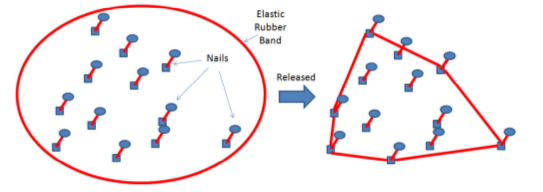
\includegraphics[width=.8\textwidth]{../img/convexhull_halim}
    \end{center}


    \begin{block}{}
      The main algorithm for calculating the convex hull is
      \emph{Graham's Scan}.

      \medskip

      It's idea is to test each point angle order, to see if the point
      belongs to the hull.
    \end{block}
  }
\end{frame}

\begin{frame}[fragile]
  \frametitle{Polygon -- Graham's Scan}
  \framesubtitle{Helping Functions}

{\small
\begin{exampleblock}{}
\begin{verbatim}
point pivot(0, 0);

bool angleCmp(point a, point b) { // angle-sorting
  if (collinear(pivot, a, b)) // special case
    return dist(pivot, a) < dist(pivot, b);
  // check which one is closer to X axis
  double d1x = a.x - pivot.x, d1y = a.y - pivot.y;
  double d2x = b.x - pivot.x, d2y = b.y - pivot.y;
  return (atan2(d1y, d1x) - atan2(d2y, d2x)) < 0; }
\end{verbatim}
\end{exampleblock}
}
\end{frame}

\begin{frame}[fragile]
  \frametitle{Polygon -- Graham's Scan}
  \framesubtitle{Convex Hull -- Initializing the algorithm}

  {\small
    \begin{exampleblock}{}
\begin{verbatim}
vector<point> CH(vector<point> P) {
  int i, j, n = (int)P.size();
  // Special Case: Polygon with 3 points
  if (n <= 3) {
    if (!(P[0]==P[n-1])) P.push_back(P[0]);
    return P; }

  // Find Initial Point: Low Y or Right X
  int P0 = 0;
  for (i = 1; i < n; i++)
    if (P[i].y < P[P0].y ||
        (P[i].y == P[P0].y && P[i].x > P[P0].x))
      P0 = i;
  point temp = P[0]; P[0] = P[P0]; P[P0] = temp;
\end{verbatim}
\end{exampleblock}}
\end{frame}

\begin{frame}[fragile]
  \frametitle{Polygon -- Graham's Scan}
  \framesubtitle{Convex Hull -- More initialization}
  {\small
    \begin{exampleblock}{}

\begin{verbatim}

  // second, sort points by angle with pivot P0
  pivot = P[0];
  sort(++P.begin(), P.end(), angleCmp);

  // S holds the Convex Hull
  // We initialize it with first three points
  vector<point> S;
  S.push_back(P[n-1]);
  S.push_back(P[0]);
  S.push_back(P[1]);

  // We start on the third point
  i = 2;
\end{verbatim}

    \end{exampleblock}
  }
\end{frame}

\begin{frame}[fragile]
  \frametitle{Polygon -- Graham's Scan}
  \framesubtitle{Convex Hull -- Main Loop}

  {\small
    \begin{exampleblock}{}
\begin{verbatim}
  while (i < n) {
    j = (int)S.size()-1;

    // If the next point is left of CH, keep it.
    // Else, pop the last CH point and try again.

    if (ccw(S[j-1], S[j], P[i]))
      S.push_back(P[i++]);
    else
      S.pop_back();
    }
  return S; }
\end{verbatim}
\end{exampleblock}}
\end{frame}
%% TODO: Add polygon problem example


\section{Conclusion}

\subsection{Problem Discussion}
\begin{frame}
  \frametitle{This Week's Problems}
  \begin{itemize}
  \item Dominator
  \item Forwarding Emails
  \item Ordering
  \item Place the Guards
  \item Doves and Bombs
  \item Come and Go
  \item ACM Contest and Blackout
  \item Ancient Messages
  \end{itemize}
\end{frame}

\begin{frame}
  \frametitle{Problem Hints (0)}

  {\smaller
  \begin{block}{Library!}
    For many of these problems, you will use a lot of repeated code:
    \begin{itemize}
    \item Visited Node arrays;
    \item Adjacent lists;
    \item Parent nodes;
    \end{itemize}

    \bigskip

    Prepare a template for the most common codes you use, and
    copy-paste it whenever necessary!
  \end{block}
  \begin{block}{Tricky Cases}
    \begin{itemize}
    \item Graphs with 1 or 0 Vertex
    \item Unconnected Graphs
    \item Self Loops
    \item Double edges
    \end{itemize}
  \end{block}
  }
\end{frame}

\begin{frame}
  \frametitle{Problem Hints (1)}  
  {\smaller
    \begin{block}{Dominator}
      \begin{itemize}
        \item If All paths from 0 to node B pass through node A, then node A {\bf dominates} node B;
        \item For all pair of nodes $i,j$, output ``Y'' if $i$ {\bf dominates} $j$, or ``N'' if not;
      \end{itemize}
    \end{block}

    \bigskip

    The idea of this problem is one of ``reachability'' -- can I reach
    node $j$ if I remove node $i$ from the graph?

    \bigskip

    Note: if $j$ is not connected to ``0'', then \emph{no one dominates j}
  }
\end{frame}

\begin{frame}
  \frametitle{Problem Hints (2)}
  {\smaller
    \begin{block}{Forwarding Emails}
      Every person $i$ sends e-mail only to person $j$.
      
      \bigskip
      
      What is the longest email chain?
      
      \bigskip
      
      Where does it start?
    \end{block}
    
    \begin{itemize}
    \item How do you deal with loops?
    \item Time limit is not very large, Try to find an O(n) solution!
    \end{itemize} 
  }
\end{frame}

\begin{frame}
  \frametitle{Problem Hints (3)}
  {\smaller
    \begin{block}{Ordering}
      Print all possible Orderings of a Direct Acyclic Graph

      \bigskip

      Generalize the DAG ordering algorithm which we discussed in class.
    \end{block}
    
    \begin{block}{Palace Guards}
      \begin{itemize}
        \item How do you represent the roads and junctions as a Graph?
        \item Find a ``guard-no guard'' assignment to vertices of the
          graph.
        \item First test if a solution is possible!
      \end{itemize}
    \end{block}    
  }
\end{frame}

\begin{frame}
  \frametitle{Problem Hints (4)}
  {\smaller
    \begin{block}{Doves and Bombs}
      This problem is about finding ``critical vertices'' in a
      graph. But how do you calculate the ``pigeon value'' of a
      vertex?
    \end{block}

    \begin{block}{Come and Go}
      Straight implementation of ``Strong Connected Components''. Be
      careful with tricky graphs!
    \end{block}    
  }
\end{frame}

\begin{frame}
  \frametitle{Problem Hints (5)}
  {\smaller
    \begin{block}{ACM Contest and Blackout}
      Goal: Find the {\bf First} minimum spanning Tree and the {\bf
        Second} minimum spanning Tree
    \end{block}

    \bigskip
    
    \begin{itemize}
    \item In this class we discussed how to find the Minimum Spanning Tree      
    \item How would we find the {\bf second minimum?}
    \item Idea: Maybe if we remove some edges from the graph?
    \end{itemize}
  }
\end{frame}

\begin{frame}
  \frametitle{Problem Hints (6)}
  \begin{block}{Ancient Message -- Challenge problem!}
    Count the symbols inside an image -- order does not matter!

    \bigskip

    What is the {\bf Main} difference between the symbols?
  \end{block}
    
  \begin{itemize}
  \item The shape and size of the symbols is actually not important!
  \item Before you begin programming, discover what is the real
    difference between the symbols.
  \item Hint: The numbers ``1'', ``0'', ``8'' have the same difference.
  \end{itemize}    
\end{frame}



\end{document}
